\chapter{性能测试与结果分析}

\section{实验环境配置}

本段将简单介绍运行Plasma的必要环境配置。这包括进行性能测试的集群硬件配置,以及编译、运行Plasma所需的其他软件要求。

\subsection{天河高性能集群硬件简介}

运行测试的天河高性能集群有超过100台CPU服务器,并由100GB的Infiniband高速网络连接而成。每个CPU节点的关键配置如下所示:

\begin{table}[h]
    \centering
    \caption{天河CPU服务器硬件配置}
    \begin{tabular}{*{4}{c}}
        \toprule
        硬件组件  & 数量 & 硬件型号 & 参数配置 \\
        \midrule
        CPU  	 & 2  & Intel(R) Xeon(R) Gold 6150 & \makecell{18核 @2.7GHz \\ L1 Cache 64K \\ L2 Cache 1024K \\ L3 Cache 25344K} \\
        \midrule
        内存 	 & 12 & / & \makecell{16Gb DDR4 \\ with ECC} \\
        \midrule
    	以太网卡 & 1  & Mellanox MT27710 Family [ConnectX-4 Lx]   & 25Gb/s \\
    	IB网卡   & 1  & Mellanox MT27700 Family [ConnectX-4] & 100Gb/s \\
        \bottomrule
    \end{tabular}
    \label{tab:hardware_config}
\end{table}

每个CPU服务器配备有双路Intel至强金牌处理器。每个CPU为6通道16G内存,因此每节点内存总量为192Gb。两路处理器形成两个NUMA节点,每节点上分别挂载有一张网卡。
该型服务器的硬件拓扑图如\autoref{fig:server_block}所示:

\begin{figure}[h]
	\centering
	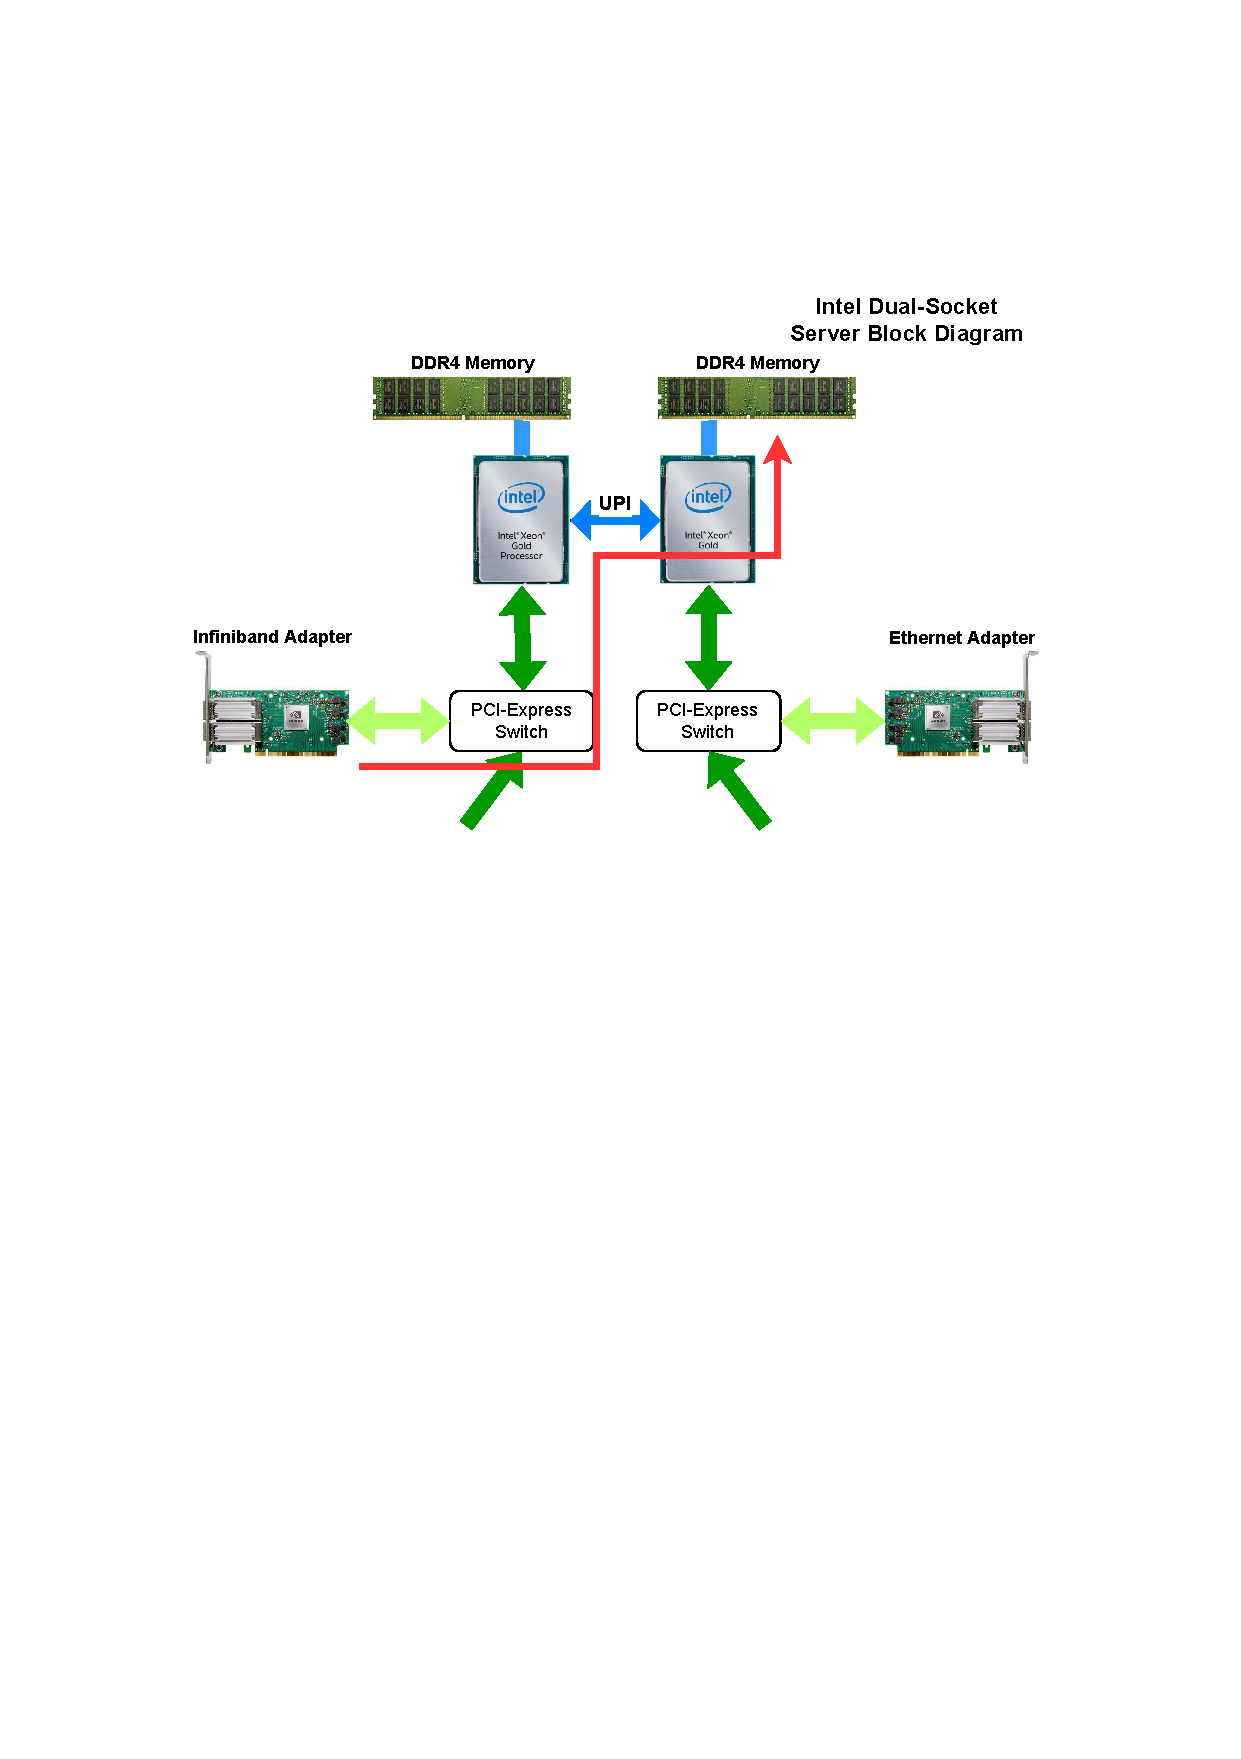
\includegraphics[width=0.7\textwidth]{image/chap04/server_block.pdf}
	\caption{天河CPU服务器硬件拓扑}
	\label{fig:server_block}
\end{figure}

需要注意的是,以太网卡和IB网卡分别挂在两个CPU的PCI-E Switch上,因而IB网卡只有在访问本NUMA节点的一半内存时拥有最佳性能——而访问远离它的CPU所控制的一半内存将会有
较大的性能损耗(\autoref{fig:server_block}中\textit{红色访存路线})。这一特性对基于RDMA的网络通信性能有明显的影响,因此在实验中需要相应调整运行配置。

\subsection{软件环境简介}

\autoref{tab:software_config}展示了本章节各性能测试所运行的软件环境。操作系统一栏展示了天河高性能集群使用的Linux操作系统版本;软件依赖指的是成功编译出可正常执行
的Plasma程序所需要的前置软件;测试软件则表示为了编译基准测试程序、运行测试程序所需要的前置软件。软件名后的数字串分别表示这些软件的版本。

\begin{table}[h]
    \centering
    \caption{天河CPU服务器软件环境}
    \begin{tabular}{*{3}{c}}
        \toprule
        软件类型 & 软件名称  & 作用描述 \\
        \midrule
        操作系统 & CentOS Linux 7 & Linux内核版本3.10.0-957.el7.x86\_64 \\
        \midrule
        \multirow{3}{*}{软件依赖} & Redis@3.2.3 & \makecell{Redis服务器存放对象在Plasma集群的分布 \\ ae事件循环库驱动Plasma进程} \\
    	 & \makecell{uthash \\ utlist \\ utarray \\ utstring}@2.0.1 & \makecell{基于宏的C语言头文件库,\\ 包装了哈希表等高级数据结构} \\
		 & gcc@9.3.0 & 编译Redis和Plasma \\
        \midrule
    	\multirow{2}{*}{测试软件} & openmpi@4.1.1 & 编译基于MPI的多节点性能测试 \\
		& hwloc@2.5.0 & 查看服务器的NUMA拓扑结构 \\
		& numactl@2.0.14 & 控制MPI进程在NUMA架构下的绑核运行 \\
        \bottomrule
    \end{tabular}
    \label{tab:software_config}
\end{table}

\section{NUMA架构下的Plasma存储测试}

\textbf{跨NUMA节点访存对性能测试的影响:}上一章节中提到了天河高性能集群存在的NUMA访问架构。IB网卡在NUMA架构中,对“远端”CPU所管理的内存发起内存访问需要通过两个CPU之间的UPI互联(The Intel Ultra Path Interconnect,\autoref{fig:server_block}中间\textit{蓝色连接}),
因而无法获得最优的访存延迟和带宽,对Plasma本地存储的性能产生较大的不利影响。由于Plasma传输数据前首先会(在发送端)访问或者(在接收端)创建内存对象,因而会进一步影响Plasma跨节点数据传输的延迟和吞吐能力。
所以,为了获得最佳的传输测试结果,我们将首先通过简单的绑核以优化Plasma的本地存储性能。

在天河高性能服务器中,通过hwloc软件提供的lstopo命令可以查看IB网卡在服务器NUMA架构中所处在的位置:以太网卡挂载在NUMA节点0上,而IB网卡挂载在NUMA节点1上。
这样,我们能通过numactl命令限制plasma\_store和plasma\_manager进程运行在NUMA节点1,从而避免IB网卡的跨NUMA节点访存。

\textbf{绑核性能测试:}为了展示绑核对访存性能的影响,我们分别在绑核与未绑核的情况下测试了Plasma本地存储操作的性能,并进行了对比。结果如\autoref{fig:numa}所示。很显然,不论是本地读还是本地写
使用绑核操作后Plasma的程序性能都有了相当明显的提升:不过,绑核运行时的写入性能随着数据增大逐渐下降,最后和不绑核时持平。可以看到,在写入较小对象时使用绑核能获得显著的性能提升,此时绑核的Plasma进程可以获得1.5倍的吞吐能力;
在读取和删除对象操作上,绑核在所有数据大小上都有显著的优化效果,其中读取操作的吞吐率增加到原来的至多1.55倍,删除操作的吞吐率增加到原来的至多5倍。

\begin{figure}[h]
    \begin{subfigure}{0.33\textwidth}
        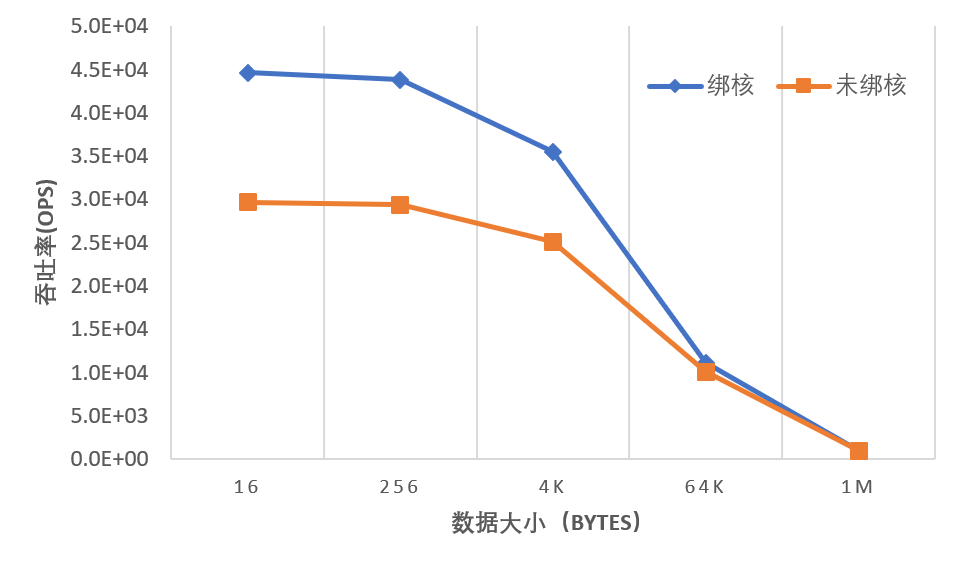
\includegraphics[width=\textwidth]{image/chap04/put.png}
        \caption{Put}
    \end{subfigure}
    \begin{subfigure}{0.33\textwidth}
        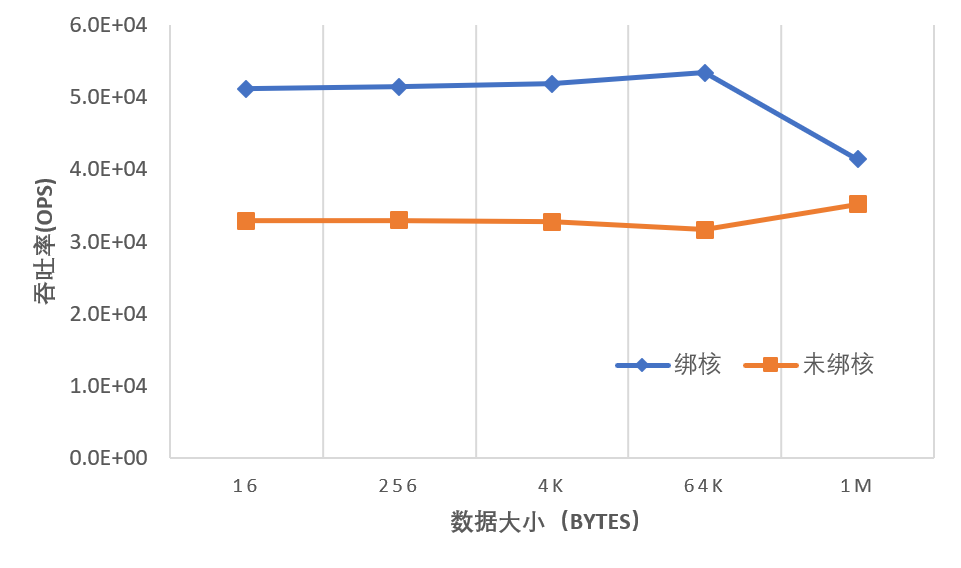
\includegraphics[width=\textwidth]{image/chap04/get.png}
        \caption{Get}
    \end{subfigure}
    \begin{subfigure}{0.33\textwidth}
        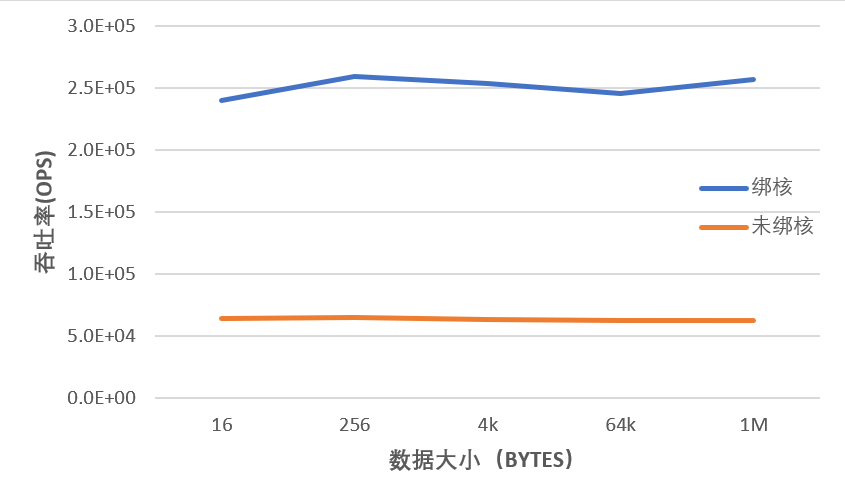
\includegraphics[width=\textwidth]{image/chap04/del.png}
        \caption{Delete}
    \end{subfigure}
    \caption{绑核对Plasma常见操作吞吐影响}
    \label{fig:numa}
\end{figure}

由于本地访存的延迟大大降低,且传输过程包括了本地访存操作,因此绑核情况下的多节点传输测试更能够体现出基于RDMA的网络协议在传输性能上的优势。
在之后的性能测试中,基于套接字以及RDMA的传输协议都将以绑核状态运行。

\section{Plasma网络协议测试}

\section{实验结果分析}